\documentclass{standalone}
\usepackage{chez}

\begin{document}
\chapter{October 13, 2020}

\begin{lemma}
  Let
  \[
    \begin{tikzcd}
    	0 \ar[r] &
    	A \ar[r] &
    	B \ar[r] &
    	C \ar[r] &
    	0
    \end{tikzcd}
  \]
  be a short exact sequence of finitely generated abelian groups.
  Then \(\rank B = \rank A + \rank C\).
\end{lemma}
We will prove a variant of this on the problem set.

Now we can prove \(\chi(X) = \sum_k (-1)^k \rank H_k(X)\).
\begin{proof}
  Consider, for all \(k \geq 0\), there are short exact sequences
  \[
    \begin{tikzcd}
    	0 \ar[r] &
    	Z^{\text{cell}}_k(X) \ar[r] &
    	\Ccell_k(X) \ar[r, "\partial"] &
    	B^{\text{cell}}_{k-1}(X) \ar[r] &
    	0
    \end{tikzcd}
  \]
  Indeed, it is exact at \(Z^{\text{cell}}_k(X)\) because the map
  \(Z^{\text{cell}}_k(X) \to C^{\text{cell}}_k(X)\) is injective, since the cycles of \(X\) are
  a subset of the chains of \(X\).
  Moreover, it is exact at \(C^{\text{cell}}_k(X)\) because the
  chains are precisely the elements in kernel of the boundary map \(\partial\).
  Then, the boundaries are defined do be the image of the boundary map,
  so \(\partial\) is surjective and the sequence is exact at
  \(B^{\text{cell}}_{k-1}(X)\).

  There is another short exact sequence
  \[
    \begin{tikzcd}
    	0 \ar[r] &
    	B^{\text{cell}}_k(X) \ar[r] &
    	Z^{\text{cell}}_k(X) \ar[r] &
    	H_k(X) \ar[r] &
    	0
    \end{tikzcd}
  \]
  It's exact at \(B^{\text{cell}}_k(X)\) because
  \(B^{\text{cell}}_k(X) \to Z^{\text{cell}}_k(X)\) is an injection,
  which is equivalent to the fact that every boundary is a cycle,
  i.e.\ \(\partial^2 = 0\).
  Also, we know that \(H_k(X)\) is the quotient of \(Z^{\text{cell}}_k(X)\)
  by \(B^{\text{cell}}_k(X)\) by definition, so the sequence
  is exact at \(Z^{\text{cell}}_k(X)\) and \(H_k(X)\).

  Using these short exact sequences, we know
  \begin{align*}
    \sum_k (-1)^k \size{I_k}
      &= \sum_k (-1)^k \rank (C^{\text{cell}}_k(X)) \\
      &= \sum_k (-1)^k (
        \rank (Z^{\text{cell}}_k(X)) + \rank (B^{\text{cell}}_{k-1}(X))
      ) \\
      &= \sum_k (-1)^k (
        \rank (B^{\text{cell}}_k(X))
        + \rank (H_k(X))
        + \rank (B^{\text{cell}}_{k-1}(X))
      ).
  \intertext{Note that the \(B^{\text{cell}}_k(X)\) terms telescope, so}
      &= \sum_k (-1)^k (\rank (H_k(X))). \pog
  \end{align*}
\end{proof}

\section{Homology with coefficients}
Another invariant easier to compute than homology is
\vocab{homology with coefficients}.
When defining homology, we applied the free abelian group functor
on the simplices of a semisimplicial set.
But one does not need to use this specific functor.
There are other functors that we can choose.
\begin{definition}
  Let \(R\) be a commutative ring and \(X\) be a semisimplicial set.
  For any \(k \geq 0\), let \(S_k(X; R)\),
  read ``\(S_k\) of \(X\) with coefficients in \(R\)'',
  to be the free \(R\)-module generated by \(X_k\).

  Let \(R\) be a commutative ring and \(X\) be a topological space.
  We can similarly define \(S_k(X, R)\) to be the free \(R\)-module
  generated by \(\Sing_k(X)\).
\end{definition}
Note that \(S_k(X, \ZZ) = S_k(X)\) because \(\ZZ\)-modules are
the same thing as abelian groups.

In both cases, whether we're dealing with semisimplicial sets
or topological spaces, the alternating sum of the semisimplicial face maps
creates the differential in a chain complex \(S_k(X; R)\).
In particular, the chain complex is of \(R\)-modules where
the differentials are \(R\)-module maps.

\begin{example}
  Consider the following semisimplicial set:
  \begin{center}
    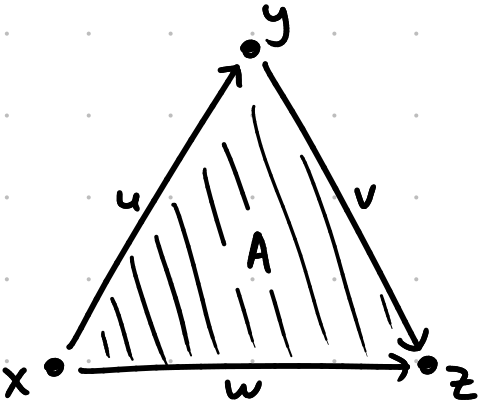
\includegraphics[width=0.2\textwidth]{18_905-201013-1.png}
  \end{center}
  Then \(S_*(X; \QQ)\) is a chain complex of rational vector spaces
  and linear maps isomorphic to
  \[
    \begin{tikzcd}
    	\cdots \ar[r] &
    	0 \ar[r] &
    	\QQ \ar[r] &
    	\QQ \oplus \QQ \oplus \QQ \ar[r] &
    	\QQ \ar[r] &
    	0 \ar[r] &
    	\cdots
    \end{tikzcd}
  \]
  where the nonzero vector spaces have bases \(\set{A}\), \(\set{u, v, w}\),
  and \(\set{x, y, z}\) respectively.
  The maps are the maps that we expect
  \[
    \begin{aligned}[t]
      \QQ & \to \QQ \oplus \QQ \oplus \QQ \\[-1ex]
      A &\mapsto u + v - w
    \end{aligned}
    \qquad
    \begin{aligned}[t]
      \QQ \oplus \QQ \oplus \QQ & \to \QQ \\[-1ex]
      u &\mapsto y - x \\[-1ex]
      v &\mapsto z - y \\[-1ex]
      w &\mapsto z - x.
    \end{aligned}
  \]
\end{example}

The homology \(R\)-modules of \(S_*(X; R)\) are denoted by \(H_q(X; R)\).
Homology with coefficients in a commutative ring satisfies all of
the Eilenberg-Steenrod axioms where the dimension axiom is modified to say
\[
  H_q(*; R) = \begin{cases*}
    R & if \(q = 0\) \\[-1ex]
    0 & otherwise.
  \end{cases*}
\]

All of the theory we've built up to calculate homology works with
homology with coefficients, so if \(X\) is a CW complex,
we can also calculate \(H_q(X; R)\) using the cellular chain complex
\(C^{\text{cell}}_*(X; R)\).

\begin{example}
  Let's consider \(\RP^2\) with the CW structure with
    one \(0\)-cell,
    one \(1\)-cell, and
    one \(2\)-cell.
  We calculated \(H_q(\RP^2) = H_q(\RP^2; \ZZ)\) with the
  cellular chain complex
  \[
    \begin{tikzcd}
    	\cdots \ar[r] &
    	0 \ar[r] &
    	\ZZ \ar[r, "2"] &
    	\ZZ \ar[r, "0"] &
    	\ZZ \ar[r] &
    	0 \ar[r] &
    	\cdots
    \end{tikzcd}
  \]
  In particular we calculated
  \[
    H_q(\RP^2) = \begin{cases*}
      \ZZ & if \(q = 0\) \\[-1ex]
      \ZZ/2\ZZ & if \(q = 1\) \\[-1ex] % chktex 1
      0 & otherwise.
    \end{cases*}
  \]
  We can also calculate \(H_q(\RP^2; \QQ)\) with the cellular chain complex
  \[
    \begin{tikzcd}
    	\cdots \ar[r] &
    	0 \ar[r] &
    	\QQ \ar[r, "2"] &
    	\QQ \ar[r, "0"] &
    	\QQ \ar[r] &
    	0 \ar[r] &
    	\cdots
    \end{tikzcd}
  \]
  Then we have the homology
  \[
    H_q(\RP^2) = \begin{cases*}
      \QQ & if \(q = 0\) \\[-1ex]
      \ZZ/2\ZZ \iso 0 & if \(q = 1\) \\[-1ex] % chktex 1
      0 & otherwise.
    \end{cases*}
  \]
  We can also calculate \(H_q(\RP^2; \FF_2)\). We have the chain
  \[
    \begin{tikzcd}
    	\cdots \ar[r] &
    	0 \ar[r] &
    	\FF_2 \ar[r, "2"] &
    	\FF_2 \ar[r, "0"] &
    	\FF_2 \ar[r] &
    	0 \ar[r] &
    	\cdots
    \end{tikzcd}
  \]
  This gives the homology
  \[
    H_q(\RP^2; \FF_2) = \begin{cases*}
      \FF_2 & if \(q = 0, 1, 2\) \\[-1ex]
      0 & otherwise.
    \end{cases*}
  \]
\end{example}

\begin{note}
  All subsequent material will not be tested until after November 9th.
\end{note}

We have covered the main ideas of homology.
However, there are more things we can ask about.
\begin{question}
  In what sense is \(H_q(X; R)\) easier than \(H_q(X; \ZZ)\)?
  Is \(H_q(X; R)\) determined by \(H_q(X; \ZZ)\)?
\end{question}
It turns out that the answer to the second question is yes.

\begin{note}
  In applied topology, one is given a giant collection of points in,
  e.g.\ \(\RR^{100}\). Fix a radius \(R\) and connect any two points
  within \(R\) apart, draw a \(2\)-simplex for all points which are in some
  diameter \(R\) circle, etc.
  We get a simplicial complex.
  We can compute the homology, and it turns out that using \(\QQ\) coefficients
  as opposed to \(\ZZ\) has much lower computational complexity.
\end{note}

\begin{question}
  How do we compute \(H_q(X \times Y)\) in terms of \(H_q(X)\) and \(H_q(Y)\)?
\end{question}

\begin{question}
  A topological space \(X\) has a diagonal map
  \(\Delta \colon X \to X \times X\) mapping \(x \mapsto (X, X)\).
  What can we say about \(H_q(\Delta X)\)?
\end{question}

\begin{question}
  What special features are enjoyed by the homology groups of manifolds
  as opposed to generic topological spaces?
\end{question}

On the way to answering these questions,
we will introduce the purely algebraic functors \(\Tor\), \(\Ext\),
and cohomology.





\end{document}
